\documentclass{beamer} 

\definecolor{blue1}{RGB}{197,229,240} % blue of figures

%\newcommand{\LinkToMethodo}{
%\begin{textblock}{25}(92,89)
%  \hyperlink{METHODO}{\beamergotobutton{Back to methodology}}
% \end{textblock}
%} 

\graphicspath{{./fig/}}


% *** TPT STYLE with added Lip6 logo ***

\definecolor{colorframetitle}{RGB}{191,18,56} % Title of frames
\definecolor{redbox}{RGB}{191,18,56} % 
\definecolor{blackbox}{RGB}{0,0,0} % 
\definecolor{brownbox}{RGB}{128,99,90} % 
\definecolor{bluebox}{RGB}{0,0,128} % 

\usepackage[absolute,overlay]{textpos}
\usepackage{listings}
\usepackage{hyperref}

\setlength{\TPHorizModule}{1mm}
\setlength{\TPVertModule}{1mm}

\usepackage{tikz}
\usetikzlibrary{decorations.pathreplacing,calc}
\usetikzlibrary{arrows,shapes,decorations,automata,backgrounds,petri}
\usepackage{scalefnt}

\newcommand{\tikzmark}[1]{\tikz[overlay,remember picture] \node (#1) {};}

\tikzstyle{mybox} = [draw=redbox, fill=redbox!20, very thick,
    rectangle, rounded corners, inner sep=10pt, inner ysep=20pt]
\tikzstyle{fancytitle} =[fill=redbox, text=white, rectangle]


\newcommand{\MyLogo}{
%\begin{textblock}{14}(117.2,0.7)
\begin{textblock}{14}(110.8,87.5)
  
\includegraphics[width=0.8cm]{tpt}
 
\includegraphics[width=0.9cm]{logo_lip6}
 \end{textblock}
}

\usepackage{beamerthemesplit}
\useoutertheme[subsection=false]{smoothbars}
\setbeamercolor{subsection in head}{parent=blue}
%\useoutertheme{miniframes}

\setbeamercolor{itemize item}{fg=redbox}
\setbeamercolor{structure}{fg=redbox, bg=red}
\setbeamercolor{block title}{bg=bluebox,fg=white}
\setbeamercolor{block title alerted}{bg=redbox,fg=white}
\setbeamercolor{block body alerted}{bg=bluebox!0,fg=black}
\setbeamercolor{block title example}{bg=black, fg=white}
\setbeamercolor{palette primary}{fg=black,bg=white} % changed this
\setbeamercolor{palette secondary}{use=structure,fg=structure.fg!100!white} % changed this
\setbeamercolor{palette tertiary}{use=structure,fg=structure.fg!100!white} % changed this
\setbeamercolor*{palette quaternary}{fg=black,bg=white} % outline on top left
\setbeamercolor{background canvas}{bg=white, fg=black} 
\setbeamercolor{frametitle}{fg=colorframetitle}

\setbeamercolor{structure}{fg=redbox, bg=redbox!70}
\setbeamercolor{structure}{fg=redbox, bg=black}
%\setbeamercolor{block title}{bg=redbox,fg=black}
\setbeamercolor{block title}{bg=black!20,fg=redbox}
\setbeamercolor{block title alerted}{bg=redbox,fg=black}
\setbeamercolor{block body alerted}{bg=redbox,fg=white}
\setbeamercolor{block title example}{bg=black!20}


% First  frame
\newcommand{\RectanglesOfMainSlide}{%
\raisebox{0mm}[0pt][0pt]{%
\begin{pgfpicture}{0mm}{0mm}{0mm}{0mm}
\pgfsetlinewidth{5mm}
\color{redbox}
\pgfline{\pgfpoint{-4mm}{-12mm}}{\pgfpoint{24mm}{-12mm}}
\color{blackbox}
\pgfline{\pgfpoint{24mm}{-12mm}}{\pgfpoint{52mm}{-12mm}}
\color{bluebox}
\pgfline{\pgfpoint{52mm}{-12mm}}{\pgfpoint{80mm}{-12mm}}
\end{pgfpicture}}}

\newcommand{\makeFirstFrame}{
\setbeamertemplate{footline}{} 
\frame[plain]{
\begin{columns}[c]
\column{3cm}
\vspace{-2cm}\\

\includegraphics[width=2.5cm]{tpt}
\\Institut\\ Mines-Telecom

\includegraphics[width=2.5cm]{fig/logo_lip6.png}
\\Paris Sorbonne University
\column{7cm}
\vspace{1cm}\\
\LARGE{\textbf{\theTitle}}\\
\vspace{0.5cm}
\normalsize{\theAuthors}\\
\vspace{0.5cm}
\normalsize{\theConferenceAndPlace}\\
\vspace{-1cm}
\RectanglesOfMainSlide
\end{columns}
}
\activateFootline
}


% Frames decoration

\newcommand{\RectanglesBeforeTitle}{%
\raisebox{0mm}[0pt][0pt]{%
\begin{pgfpicture}{0mm}{0mm}{0mm}{0mm}
\pgfsetlinewidth{5mm}
\color{redbox}
\pgfline{\pgfpoint{-2mm}{2.2mm}}{\pgfpoint{4mm}{2.2mm}}
\color{blackbox}
\pgfline{\pgfpoint{4mm}{2.2mm}}{\pgfpoint{10mm}{2.2mm}}
\color{bluebox}
\pgfline{\pgfpoint{10mm}{2.2mm}}{\pgfpoint{16mm}{2.2mm}}
\end{pgfpicture}}}

\setbeamertemplate{frametitle}{
\begin{columns}[t]
\column{16mm}
\RectanglesBeforeTitle 
\column{10.7cm}
\strut\textbf{\insertframetitle}\strut
\end{columns}
}

% Foot line

\newcommand{\Ffootline}{
\MyLogo
\begin{tikzpicture}
 \fill [color=white, fill=redbox] (-1, -0.05) rectangle (1, 0.30);
\node[white, right] (note1) at (-1, 0.10) {\insertframenumber/\inserttotalframenumber};
%\node[white, left] (note1bis) at (0.98, 0.10) {\theDate};
\node[white, left] (note1bis) at (1.05, 0.10) {\theDate};
% \fill [color=white, fill=blackbox] (1.05, -0.05) rectangle (4.5, 0.30);
 \fill [color=white, fill=blackbox] (1.05, -0.05) rectangle (6.5, 0.30);
\node[white, align=center] (note2) at (3.77, 0.12) {Institut Mines-Telecom, Paris Sorbonne Universites};
% \fill [color=red, fill=bluebox] (4.55, -0.05) rectangle (10.75, 0.30);
\fill [color=red, fill=bluebox] (6.55, -0.05) rectangle (10.75, 0.30);
\node[white, align = center] (note3) at (8.15, 0.10) {\footnoteTitle};
%
\includegraphics[width=1]{fig/logo_lip6.png}
%\node[white] (note3) at (7.5, 0.10) {\theTitle};
\end{tikzpicture}
%
\includegraphics[width=1cm]{logo_lip6}
}

\newcommand{\activateFootline}{
\setbeamertemplate{footline}{
\usebeamerfont{structure}
\Ffootline
}
}


% *** END OF TPT STYLE ***


%remove navigation symbols
\setbeamertemplate{navigation symbols}{}

% To show the outline at the beginning of each section
%\AtBeginSection[]{
%   \begin{frame}
%   \frametitle{Outline}
%   %\begin{center}{\LARGE Outline }\end{center}
%   \tableofcontents[currentsection,hideothersubsections]
%   \end{frame} 
%}

%\newcommand{\LinkToMethodo}{
%\begin{textblock}{25}(102,89)
%  \hyperlink{METHODO}{\beamergotobutton{Back to methodology}}
% \end{textblock}
%}

\lstset{language=C,basicstyle=\tiny,keywordstyle=\color{red}\bfseries,  commentstyle=\color{blue}\textit,stringstyle=\color{green}\ttfamily, showspaces=false,showstringspaces=false}

\newcommand{\mytilde}{\raise.17ex\hbox{$\scriptstyle\mathtt{\sim}$}}

\newcommand{\tikzgrid}{
\begin{pgfonlayer}{background}
\draw[gray!50]
(current bounding box.south west)
grid[step=.2] (current bounding box.north east);
\draw[red!50]
(current bounding box.south west)
grid (current bounding box.north east);
\end{pgfonlayer}
}

\newcommand*{\ExtractCoordinate}[3]{\path (#1); \pgfgetlastxy{#2}{#3};}%

\newdimen\tlx
\newdimen\tlx
\newdimen\brx
\newdimen\bry




\newcommand{\footnoteTitle}{Using TTool with SoCLib}
\newcommand{\theTitle}{\normalsize{Using TTool with SoCLib}}
\newcommand{\theAuthors}{Daniela Genius, Ludovic Apvrille\\daniela.genius@lip6.fr\\ ludovic.apvrille@telecom-paristech.fr}
\newcommand{\theConferenceAndPlace}{Users' Guide to the \\\textbf{SoCLib} extension\\ of \textbf{TTool/AVATAR}}
\newcommand{\theDate}{February 2016}

\graphicspath{{./fig/}}


\definecolor{color1}{rgb}{0.87,0.00,0.21} % rouge ENST
\definecolor{myblue}{rgb}{0.00,0.00,1.00} % blue for tables

\begin{document}

\makeFirstFrame



%\lstset{language=C,basicstyle=\scriptsize,keywordstyle=\color{red}\bfseries,  commentstyle=\color{blue}\textit,stringstyle=\color{green}\ttfamily,labelstyle=\tiny, showspaces=false,showstringspaces=false}

% To show the outline at the beginning of each section
%\AtBeginSection[]{
 % \begin{frame}
 %  \MyLogo
 %  \frametitle{Outline}
 %  \tableofcontents[currentsection,hideothersubsections]
  % \end{frame} 
%}
	

\setbeamercolor{background canvas}{bg=color1} 

\setbeamercolor{background canvas}{bg=white} 

\section{Compilation Tool Chain}
\subsection{Context}

\frame[containsverbatim]{
\MyLogo
\frametitle{Virtual Prototyping of AVATAR Diagrams}
\begin{block}{Diagram Editor}
\begin{itemize}
\item AVATAR 
Diagrams (existing)
\item Deployment Diagrams 
(new)
\item We do not yet consider security aspects
\end{itemize}
\end{block}
\begin{block}{Generate Code for MPSoC platform}
\begin{itemize}
\item Tasks and Main
\item Ldscript
\item Topcell
\end{itemize}
\end{block}
}




\subsection{Compilation Tool Chain}
\frame[containsverbatim]{
\MyLogo
\frametitle{Compilation Tool Chain}
\begin{columns}[c]
\column{6cm}
\begin{small}
\begin{enumerate}
\item \textbf{DDSyntaxChecker} checks syntax of deployment diagrams and identifies their elements
\item  \textbf{Libavatar} Runtime for \mbox{SoCLib}, implements \mbox{AVATAR} operators
\item \textbf{\mbox{AVATAR}2SOCLIB} translates \mbox{AVATAR} blocks into C POSIX tasks, generates main program
\item \textbf{TopcellGenerator} generates SystemC top cell 
\item \textbf{LdscriptGenerator} generates linker script
\end{enumerate}
\end{small}
\column{7cm}
\begin{center}
%Yellow: extensions to TTool
%\includegraphics[width=6cm]{toolchain-doc}
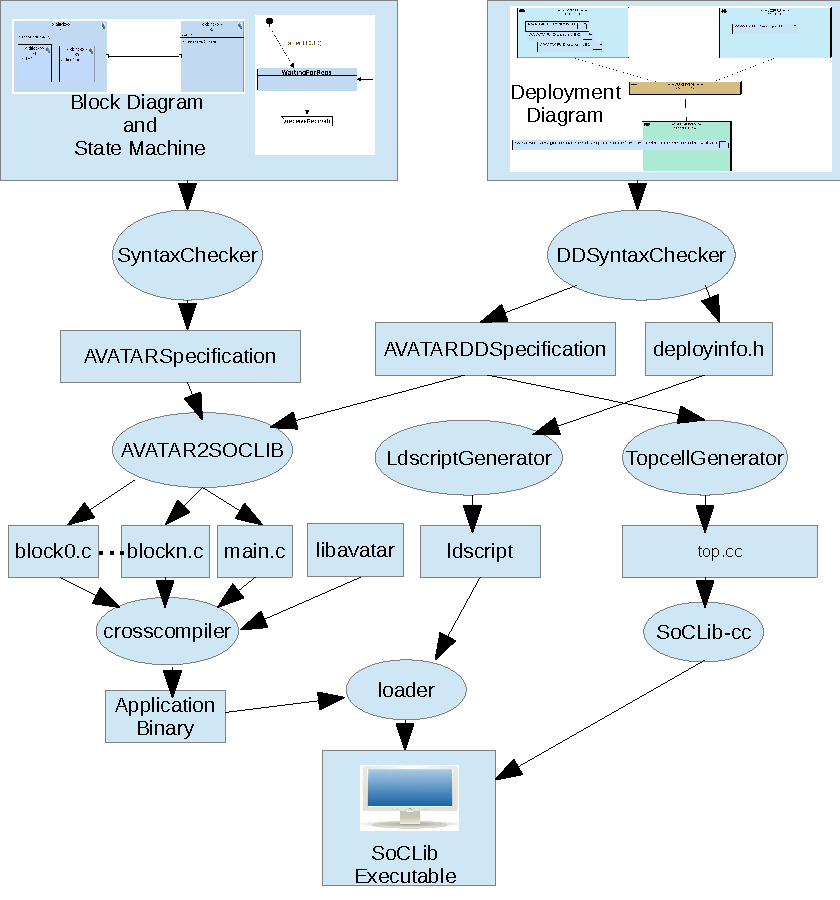
\includegraphics[width=6cm]{toolchain}
%\caption{}
\end{center}
\end{columns}
}

\subsection{Deployment Diagrams}
\frame[containsverbatim]{
\MyLogo
\frametitle{Deployment Diagrams}

\begin{itemize}
\item  SysML representation of hardware components, their interconnection, tasks and channels
\item A valid platform must contain at least one CPU, one memory bank and one terminal for observing the progress
\item Some details (interrupt controller, simulation aides) currently left transparent to the user
\end{itemize}
}


\subsection{Deployment Diagrams Screen}
\frame[containsverbatim]{
\MyLogo
\frametitle{Deployment Diagrams Screen}
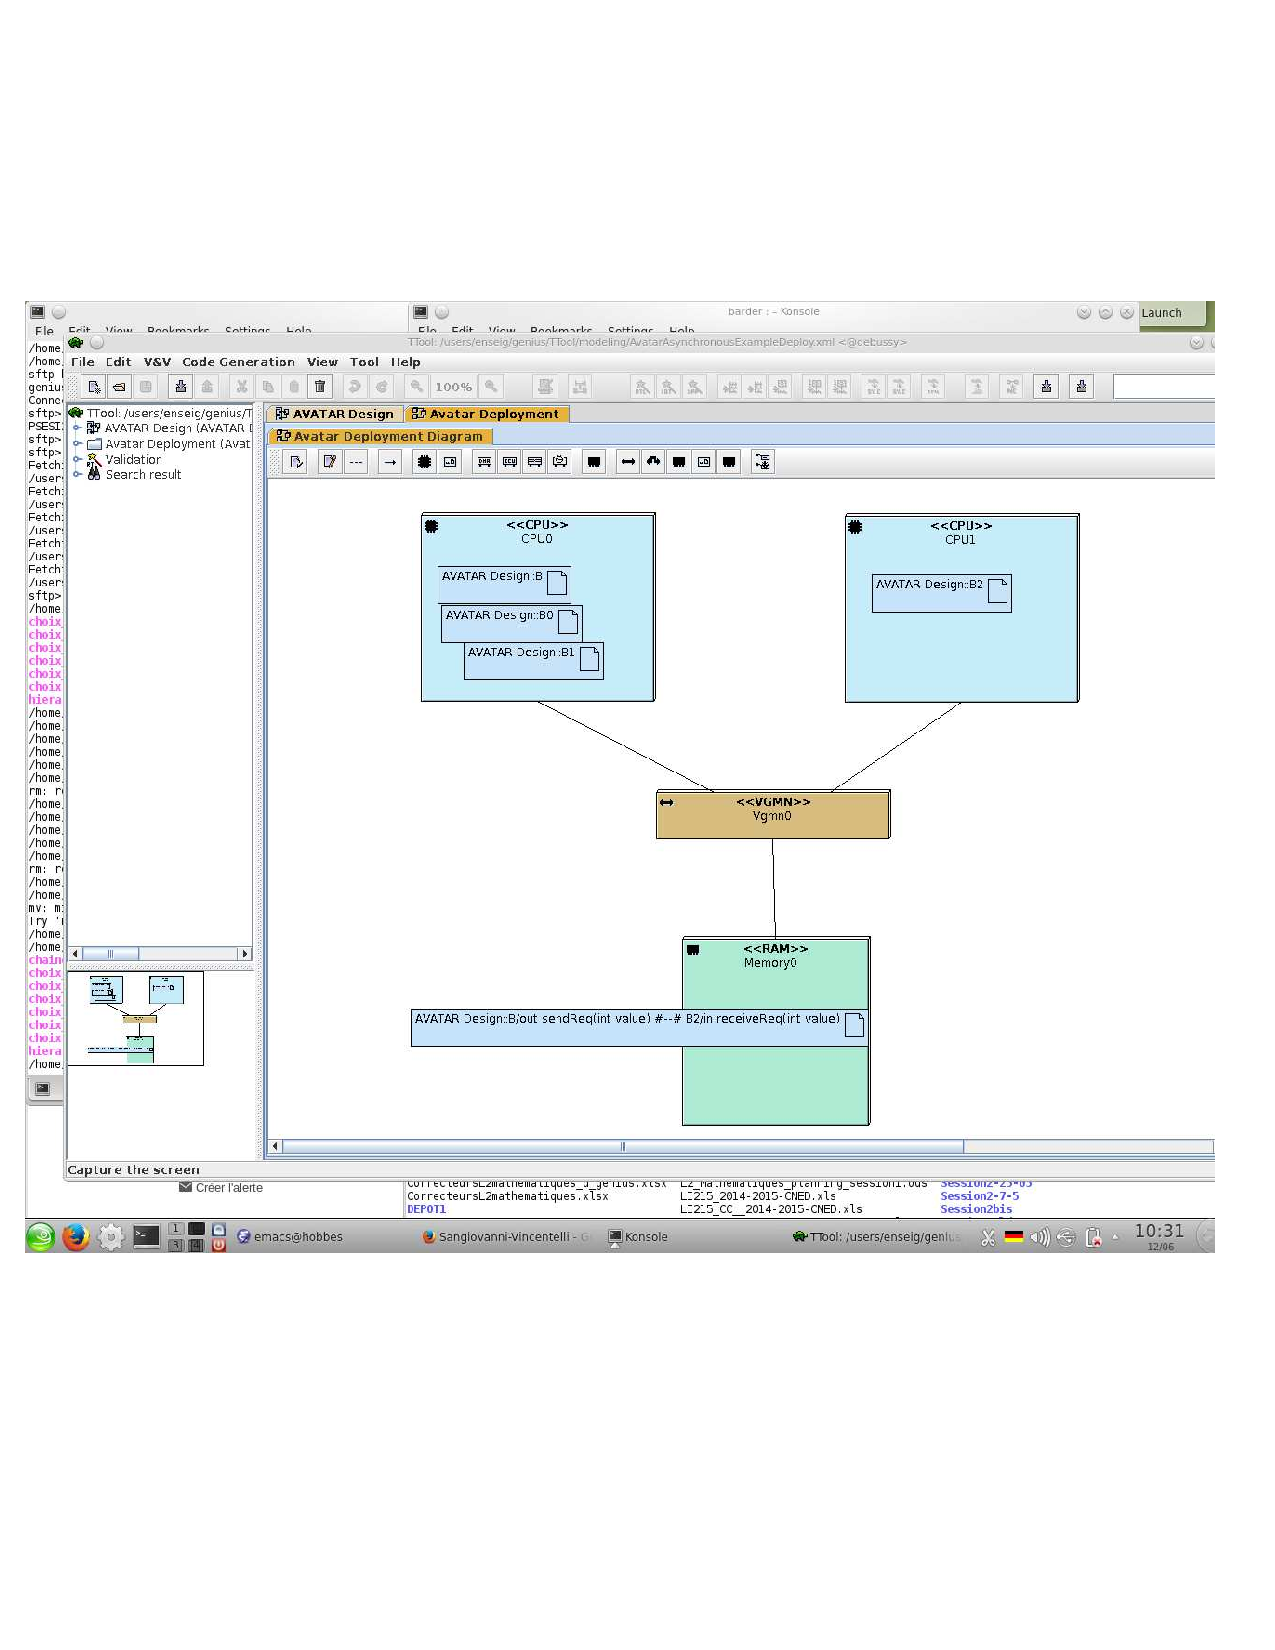
\includegraphics[width=9.5cm]{screen}
%\begin{itemize}
%\item Click on AVATAR Design (left tab)
%select V\&V (the Syntax Analysis reads in the diagrams and checks their syntax)
%\end{itemize}
}
\subsection{Deployment Diagrams Toolbar}
\frame[containsverbatim]{
\MyLogo
\frametitle{Deployment Diagrams Toolbar}
\begin{center}
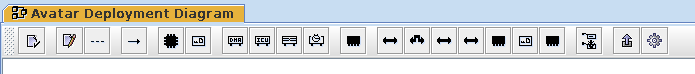
\includegraphics[width=11cm]{toolbar_deploy}
\end{center}
From left to right:
\begin{tiny}
\begin{columns}[c]
\column{6cm}
\begin{itemize}
\item Edit
\item Comment
\item UML connector
\item Link two nodes
\item Add a CPU
\item Map task to CPU
\item DMA: not yet implemented
\item ICU: currently added automatically in all platforms
\item COPROCESSOR: not yet implemented
\item TIMER: not yet implemented
\item TTY
\end{itemize}
\column{6cm}
\begin{itemize}
\item BUS
\item BRIDGE: not yet implemented
\item VGMN
\item CROSSBAR 
\item RAM
\item Map channel to RAM : map channels onto memory banks
\item ROM
\item Show/hide attributes
\item Extract attributes
\item Generate code
\end{itemize}
\end{columns}
\end{tiny}
}


\frame[containsverbatim]{
\MyLogo
\frametitle{Add a Hardware Module}
\begin{itemize}
\item 
Left click on the desired module on the toolbar, then click on screen.
\item In the example, we add a CPU.
\end{itemize}
\begin{center}
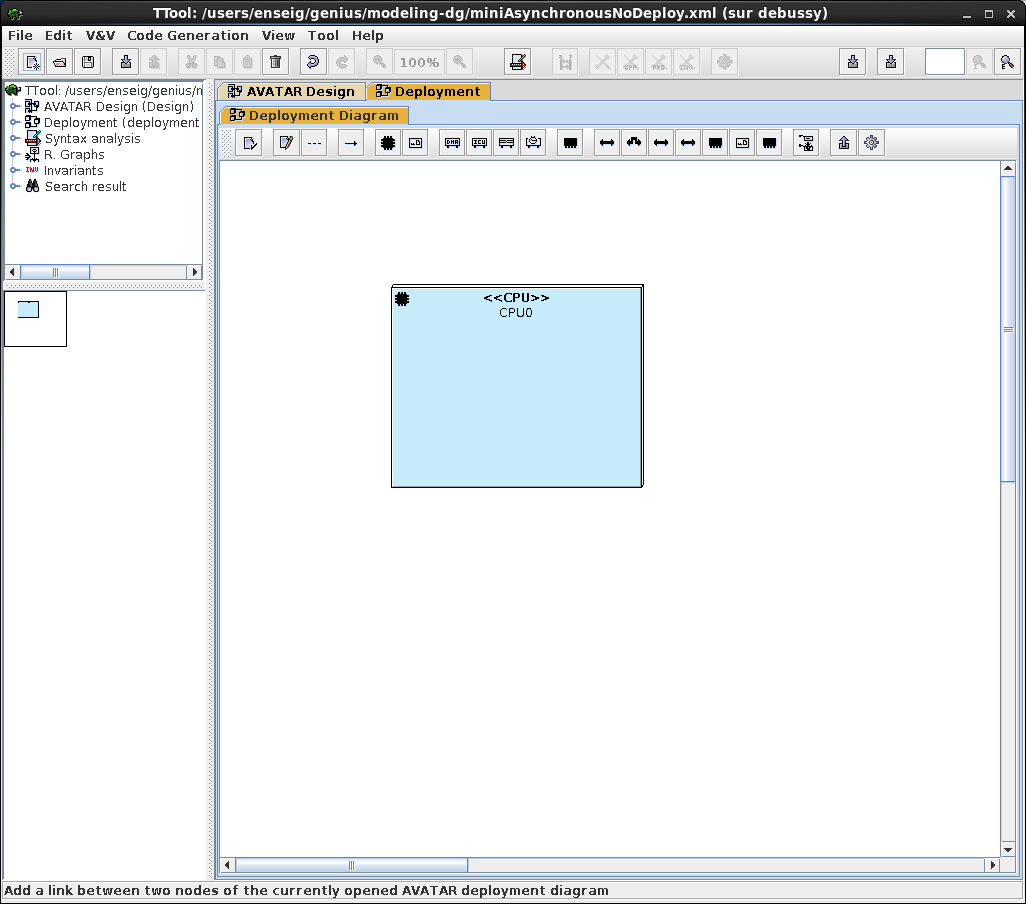
\includegraphics[width=8cm]{fig/add_module}\\

\end{center}
}

\frame[containsverbatim]{
\MyLogo
\frametitle{Modify Hardware Attributes}
\begin{itemize}
\item 
Right click on components then select \textbf{edit} allows to modify attributes : e.g. specify number of cache lines,
the size of memory bank

\begin{center}
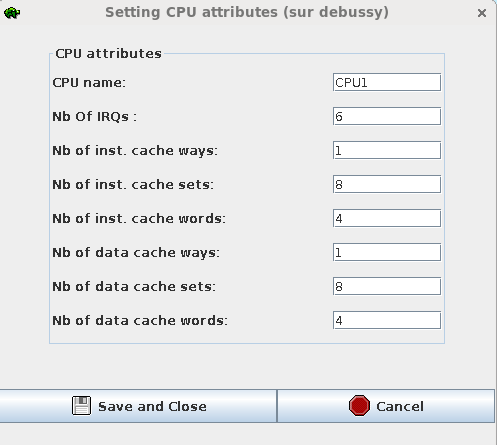
\includegraphics[width=6cm]{fig/menu_cache}\\

Editing hardware parameters
\end{center}
\end{itemize}
}

\frame[containsverbatim]{
\MyLogo
\frametitle{Modify Hardware Attributes (cont.)}
\begin{itemize}
\item 
For a RAM, you have to specify the size, which is 0
per default
\item You also have to determine in a menu one among three choices of monitoring
\begin{itemize}
\item VCD trace (default): generates a VCD trace that can be viewed e.g. with gtkwave. File \texttt{mytrace.vcd}.
\item VCI Logger: monitors all traffic on the VCI (attention traces are very big). Output on tty
\item VCI stats: extraction tool based on the VCI logger that traces actions on channels. File \texttt{mwmr.log}.
\end{itemize}
\begin{center}
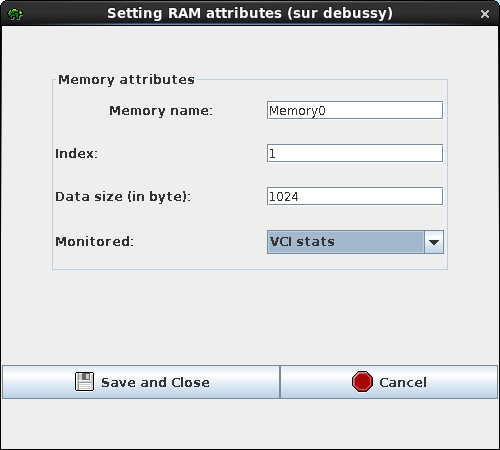
\includegraphics[width=4cm]{fig/menu_ram}\\

Editing hardware parameters
\end{center}
\end{itemize}
}
\frame[containsverbatim]{
\MyLogo
\frametitle{Modify Hardware Attributes (cont.)}
\begin{itemize}
\item 
For a VGMN interconnect, you have to set the latency to at least 3
\item The number of initiators and targets can be set, but is currently calculated automatically (as we have modules, interrupt and simulation infrastructure added transparently)
\begin{center}
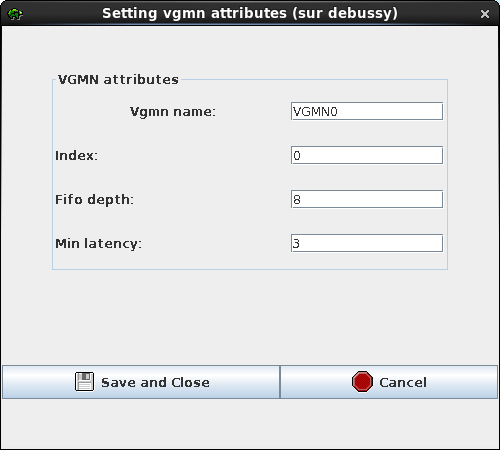
\includegraphics[width=5cm]{fig/menu_vgmn}\\

Editing hardware parameters
\end{center}
\end{itemize}
}



\frame[containsverbatim]{
\MyLogo
\frametitle{Connect Hardware Modules}
We added a second module (an interconnect). Now we wish to connect the two. For this :
\begin{itemize}
\item Left click on arrow in the tool bar.
\item Left click on starting point which becomes embossed (a module has 16 connecting points around its rim)
\item Left click on ending point point  which becomes embossed when the cursor approaches.
\item In the example, we connected a Bus and the CPU.
\item Important: you have to chose the other module first, the bus or interconnect second.
\end{itemize}

}

\frame[containsverbatim]{
\MyLogo
\frametitle{Connect Hardware Modules (Cont.)}

\begin{center}
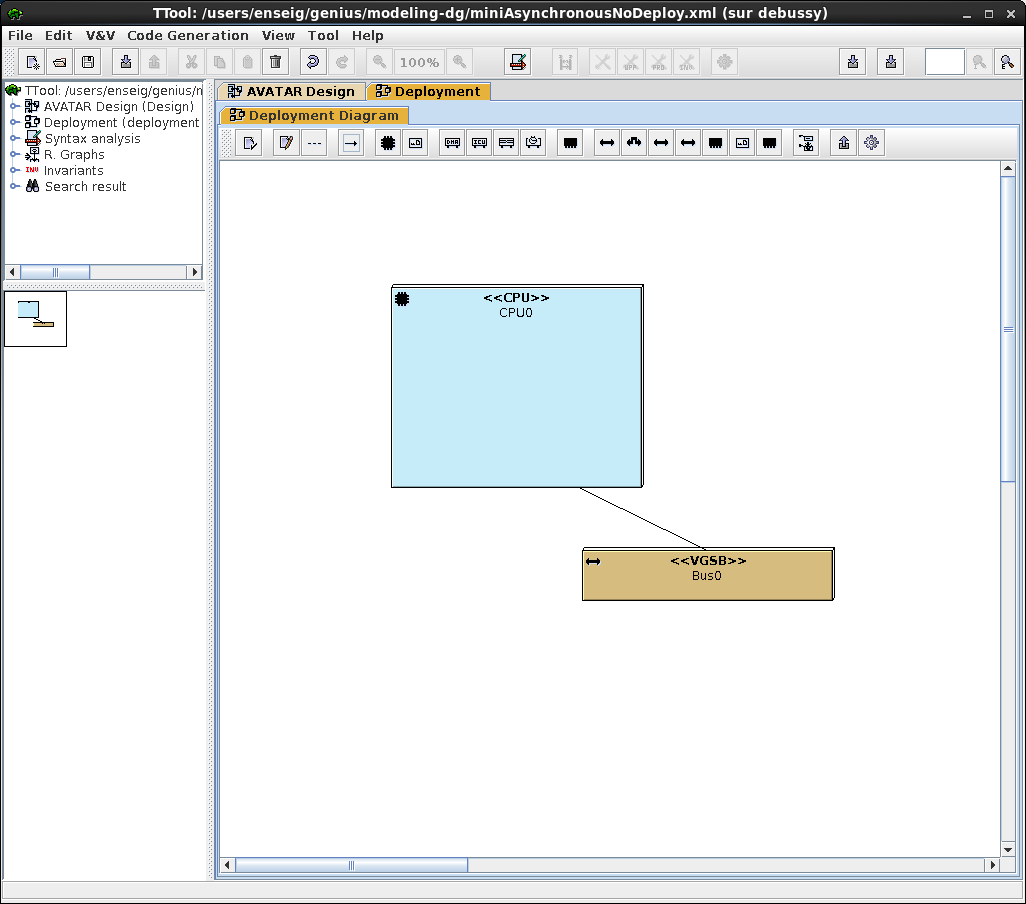
\includegraphics[width=9.5cm]{fig/connect_modules}\\

\end{center}
}

\subsection{Deployment Diagrams: Example}
\frame[containsverbatim]{
\MyLogo
\frametitle{Example}
\begin{columns}[c]
\column{5.5cm}
\begin{center}
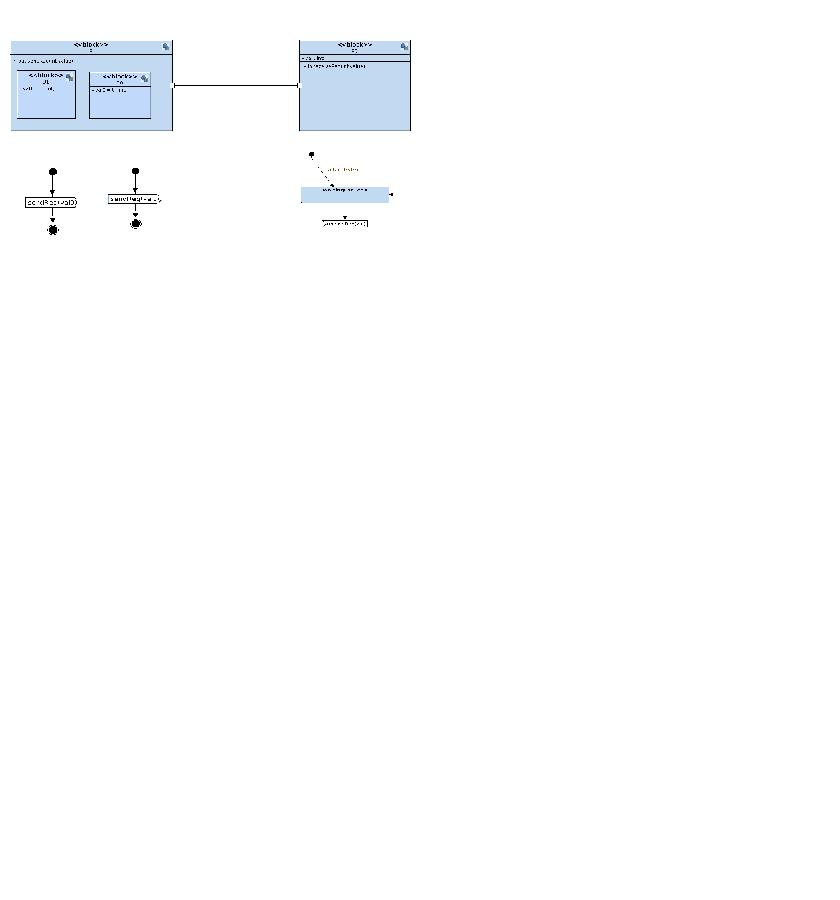
\includegraphics[width=5cm]{petit_exemple}\\
AVATAR example\\
featuring 4 blocks,\\ two of which nested,\\and one channel
\end{center}
\column{7cm}
\begin{center}
\includegraphics[width=6cm]{petit_exemple_before}\\
\end{center}
\end{columns}

}

\subsection{Deployment Diagrams: Example (cont.)}
\frame[containsverbatim]{
\MyLogo
\frametitle{Example}
\begin{columns}[c]
\column{3.5cm}
\begin{center}
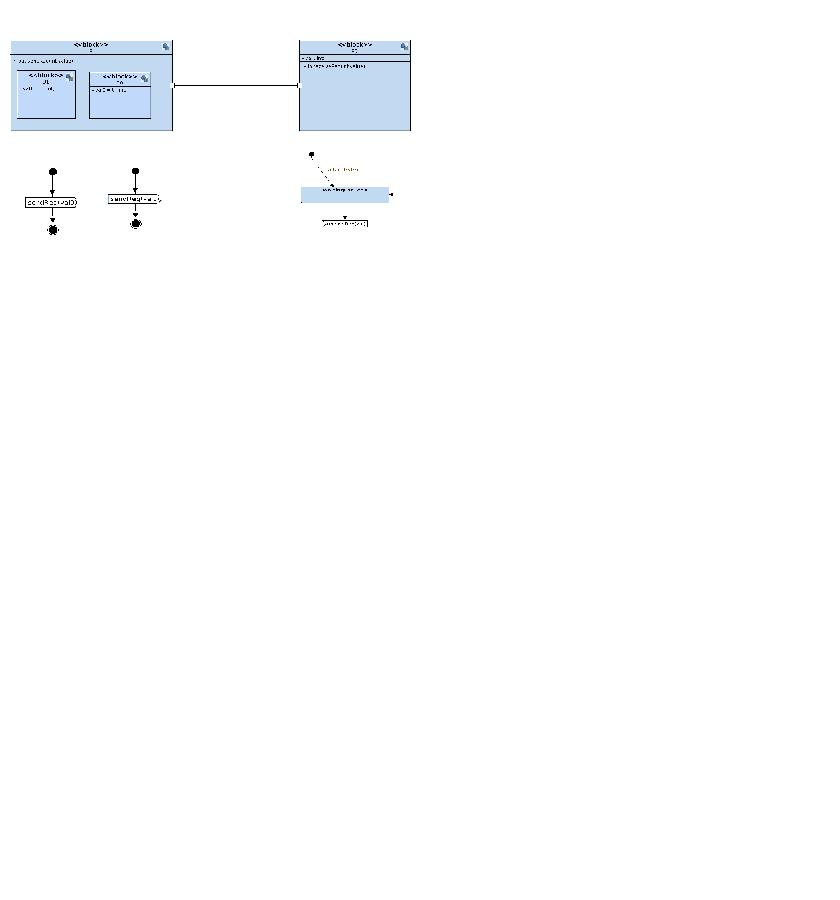
\includegraphics[width=5cm]{petit_exemple}\\
\end{center}
To map tasks on processors, click on task icon 
\includegraphics[width=0.5cm]{fig/ddartifact}\\.
Then, select Edit and choose the name of the task.\\

\column{7cm}
\begin{center}
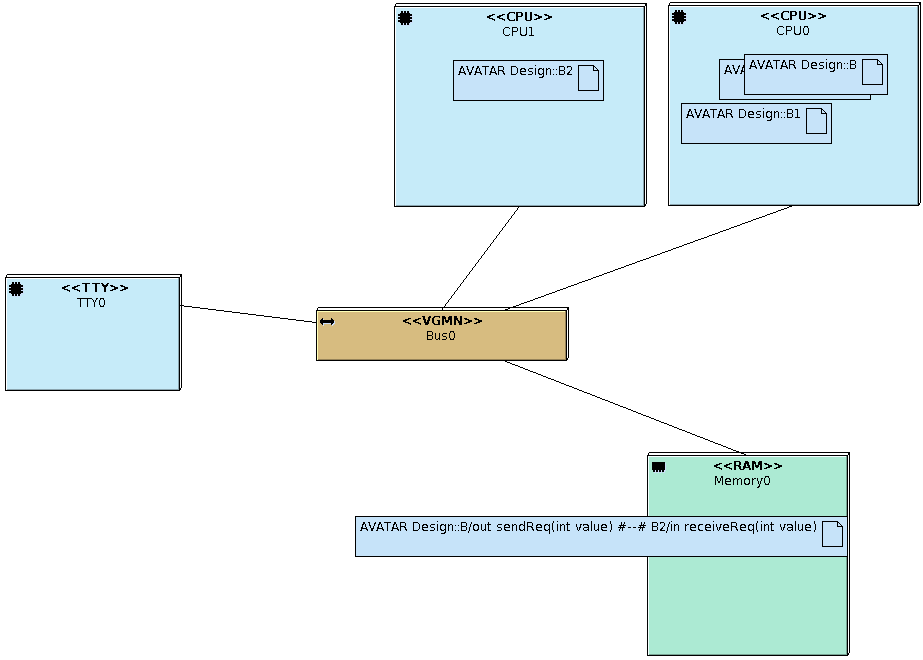
\includegraphics[width=4cm]{deployment_2RAM}\\
\end{center}
To map channels on memory banks, click on channel icon 
\includegraphics[width=0.5cm]{fig/ddartifact} (which looks the same but is located more to the right of the toolbar)\\.
Then, select Edit and choose the name of the channel.
There will be a warning on the terminal if not all tasks or channels are mapped,
listing those missing.

\end{columns}
}

\subsection{The \mbox{AVATAR} Runtime}
\frame[containsverbatim]{
\MyLogo
\frametitle{The \mbox{AVATAR} Runtime}
Library of functions which capture the semantics of the \mbox{AVATAR} operators that appear in the code of the tasks
implemented using MutekH \texttt{http://www.mutekh.org} primitives
\begin{itemize}
\item Directory \texttt{TURTLE/MPSoC/src} contains the runtime
\item \texttt{Makefile.forsoclib} with targets 
\begin{itemize}
\item \texttt{updategeneratedcode}: generated code copied into MPSoC/mutekh/examples/avatar
\item \texttt{updateruntime}: runtime copied into MPSoC/mutekh/libavatar
\end{itemize}
\end{itemize}
}


\frame[containsverbatim]{
\MyLogo
\frametitle{The \mbox{AVATAR} Runtime (2)}
Implements the semantics of  AVATAR operators
\begin{tabular}{|l|l|}\hline
\bf{Operator}&\bf{Semantics}\\\hline
Asynchronous read&Blocking\\
Asynchronous write&Blocking or non blocking\\
Synchronous read/write&Blocking\\
Delay [min..max]&Processor is suspended\\
Complexity [min..max]&Active execution \\
Test&Depends on Boolean condition\\
Non deterministic choice& The first message in the\\
&queues triggers the transition\\
& or a branch is randomly taken\\\hline
\end{tabular}
}

\frame[containsverbatim]{
\MyLogo
\frametitle{The \mbox{AVATAR} Runtime (3)}
\begin{itemize}
\item \texttt{asyncchannel}: SoCLib implementation of asynchronous channel
\item \texttt{debug}: debug functions 
\item \texttt{message}: describes one message
\item \texttt{myerrors}: error treatment
\item \texttt{mytimelib}: time functions library
\item \texttt{random}: ramdom functions
\item \texttt{request}: describes one request
\item \texttt{request\_manager}: central manager of requests
\item \texttt{syncchannel}: SoCLib implementation of synchronous channel
\item \texttt{tracemanager}: managing traces (cycle precise traces not yet implemented)
\end{itemize}
}

\subsection{Code Generation}
\frame[containsverbatim]{
\MyLogo
\frametitle{Code Generation}
\begin{center}

Generation of MPSoC code in TURTLE/MPSoC directory's subdirectories
\begin{itemize}
\item \texttt{generated\_topcell}: contains three files:
\begin{itemize}
\item \texttt{top.cc}: generated topcell, to be copied into

\texttt{MPSoC/soclib/soclib/platform/topcells/\\caba-vgmn-mutekh\_kernel\_tutorial/}

\item \texttt{nbproc}: number of processors extracted from Deployment Diagram used for ldscript generation
\item \texttt{deployinfo.h}: information on channel mapping extracted from Deployment Diagram used for ldscript generation
\end{itemize}
\item \texttt{generated\_src}: code for tasks and main program, to be copied into

\texttt{MPSoC/mutekh/exaples/avatar}
\end{itemize}
\end{center}
}


\frame[containsverbatim]{
\MyLogo
\frametitle{SystemC Top Cell Generation}
The topcell is generated and contains several parts, liste din alphabetical order:

\begin{itemize}
\item Code.java: some fixed code (gdb call etc) 
\item Declaration.java: Declaration of hardware components
\item Header.java: some fixed code
\item Loader.java: call to the loader  
\item MappingTable.java: declaration of the memory segments (shared memory architecture)
\item NetList.java: netlist, connecting signals to ports
\item Signal.java: declaration of signals used in netlist 
\item Simulation.java: call to simulation engine
\item TopCellGenerator.java: main class
\end{itemize}
}


\subsection{Top Cell Generation}
\frame[containsverbatim]{
\MyLogo
\frametitle{SystemC Top Cell Generation (2)}
The topcell is generated and contains several parts, each corresponding 
to part of its code.
Example lines from a generated topcell:
\begin{itemize}
\item Instanciation of components:
\begin{lstlisting}
soclib::caba::VciRam<vci_param>Memory0("Memory0", IntTab(2), maptab);
\end{lstlisting}
\item memory segments: 
\begin{lstlisting}
maptab.add(Segment("data", 0x7f000000, 0x01000000, IntTab(2), false)); 
\end{lstlisting}
\item charging of code:
\begin{lstlisting}
data_ldr.load_file(std::string(kernel_p) + 
  ";.data;.channel0;.cpudata;.contextdata");
\end{lstlisting}
\item Netlist: 
\begin{lstlisting}
vgsb.p_to_target[2](signal_vci_vciram0);
\end{lstlisting}
\end{itemize}
}


\subsection{Linker Script Generator}
\frame[containsverbatim]{
\MyLogo
\frametitle{Linker Script}
\begin{itemize}
\item Defines the memory layout 
\item Associates each entry section to an output section
\item \texttt{~/MPSoC/mutekh/arch/soclib} contains generator
\item copied into \texttt{~/MPSoC/mutekh/obj-avatar-soclib-ppc/arch}
\item implements the mapping of channels by forcing them on the memory bank specified in the Deployment Diagram
\end{itemize}
\begin{tiny}
\begin{center}
\begin{lstlisting}
MEMORY
{
    mem_ram (RWAL): ORIGIN = 0x7f000000, LENGTH = 0x01000000
...
}
SECTIONS
{
...
 .data : {
  __data_start = ABSOLUTE(.);
  *(.sdata*)
  *(.data*)
  *(.cpuarchdata*)
 } > mem_ram AT>mem_rom
 .channel0 : { *(section_channel0)} > mwmrd_ram
...
}
\end{lstlisting}
\end{center}
\end{tiny}
}



\section{Simulation}

\subsection{Syntax Checking}

\frame[containsverbatim]{
\MyLogo
\frametitle{Syntax Checking}
Click on the \texttt{AVATAR Design} tab (this cannot be invoked from the \texttt{AVATAR Deployment} tab)

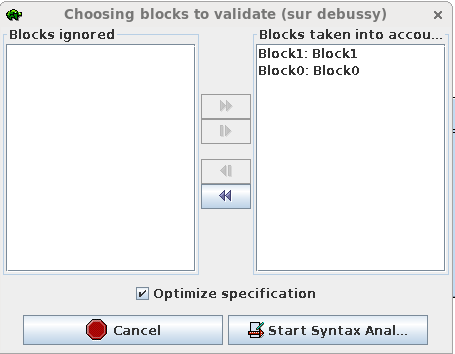
\includegraphics[width=6cm]{menu_v_and_v}

You should get a message indicating there are no errors; otherwise refer to the general TTool documentation.
}


\subsection{Code Generation Dialogue}
\frame[containsverbatim]{
\MyLogo
\frametitle{Code Generation Dialogue}
\begin{itemize}
\item Click on AvatarDeployment (right tab) 
Click on the gear at the right of the lower toolbar (Deployment Diagram Toolbar)
\item Select trace and:or debug mode if required 
\item Select \textbf{Compile soclib executable} in the compile menu
\item Select \textbf{Run code in soclib/mutekh} in the \textbf{Execute} menu
\end{itemize}
\begin{center}
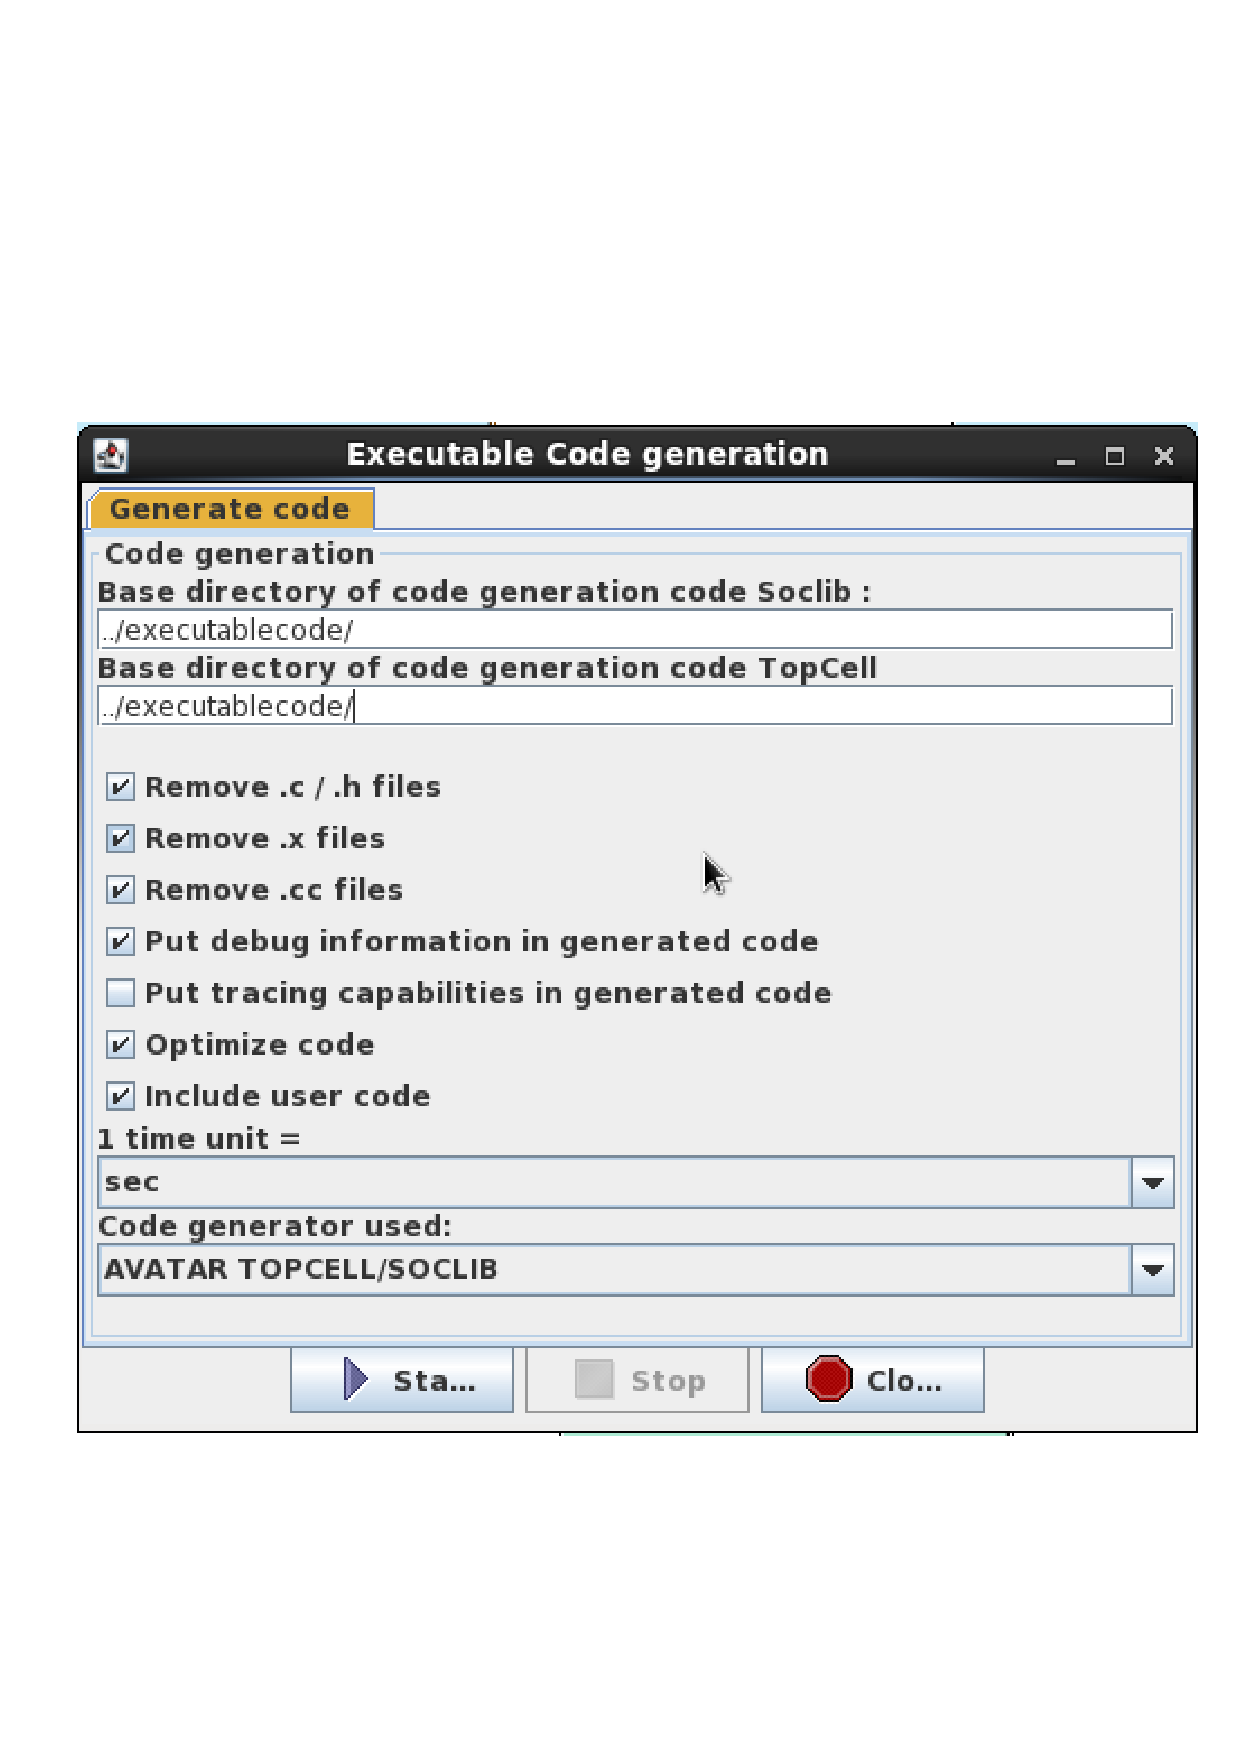
\includegraphics[width=5cm]{JDialog}
\end{center}
}


\subsection{Compilation}
\frame[containsverbatim]{
\MyLogo
\frametitle{Compilation Dialogue}
Normally, this is done by pushing the \texttt{Compile soclib executable} button in the menu below.\\

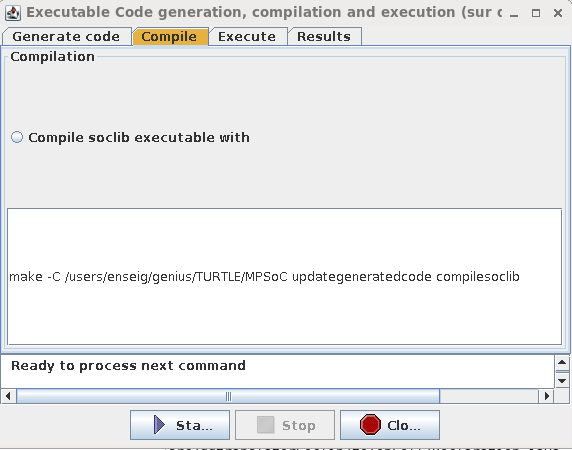
\includegraphics[width=6cm]{menu_compil}\\

}


\frame[containsverbatim]{
\MyLogo
\frametitle{Compilation (2)}
Alternatively, for test and debug purposes, you may wish to manually modify the code of task and main files. The code is copied into the following directory:
\texttt{~/MPSoC/mutekh/examples/avatar}

Type \texttt{cd ~/MPSoC/mutekh;} 

 \texttt{make CONF=examples/avatar/config BUILD=soclib-\$(MUTEKH\_CPU):pf-tutorial}

Where \texttt{MUTEKH\_CPU} is your CPU (currently ppc)

\medskip
\textbf{Be careful when you modify generated code, your changes will be lost at next code generation!}
}



\subsection{Invoking SoCLib from TTool}
\frame[containsverbatim]{
\MyLogo
\frametitle{Simulation Dialogue}
Normally, this is done by pushing the \texttt{Run code in soclib/mutekh button} in the menu (cycle accurate trace facility will be added later on)

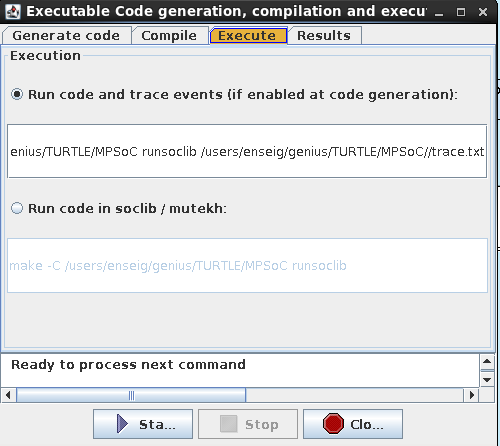
\includegraphics[width=6cm]{menu_exec}\\

}

\frame[containsverbatim]{
\MyLogo
\frametitle{Simulation (2)}
Alternatively, for test and debug, you may wish to manually modify the topcell. in this case, go to the following directory:\\ \texttt{MPSoC/soclib/soclib/platform/topcells/\\caba-vgmn-mutekh\_kernel\_tutorial/}

Eventually modify \texttt{top.cc}

Type \texttt{make}

Then start the platform executable

\texttt{./system.x \$(SOCLIB\_CPU):\$(SOCLIB\_CPU\_COUNT)\\ ~/MPSoC/mutekh/avatar-soclib-\$(MUTEKH\_CPU).out}

Where \texttt{SOCLIB\_CPU\_COUNT} has to correspond to the number of CPUs used in your Deployment Diagram and \texttt{MUTEKH\_CPU} is the type of CPU (currently ppc)
}

\subsection{Simulation}
\frame[containsverbatim]{
\MyLogo
\frametitle{Invoking SoCLib from TTool}

A TTY (green on black) should open; if the debug option was selected, the
application progress can be watched and read/write operations on channels can be monitored 
\begin{columns}[c]
\column{6cm}
\begin{center}
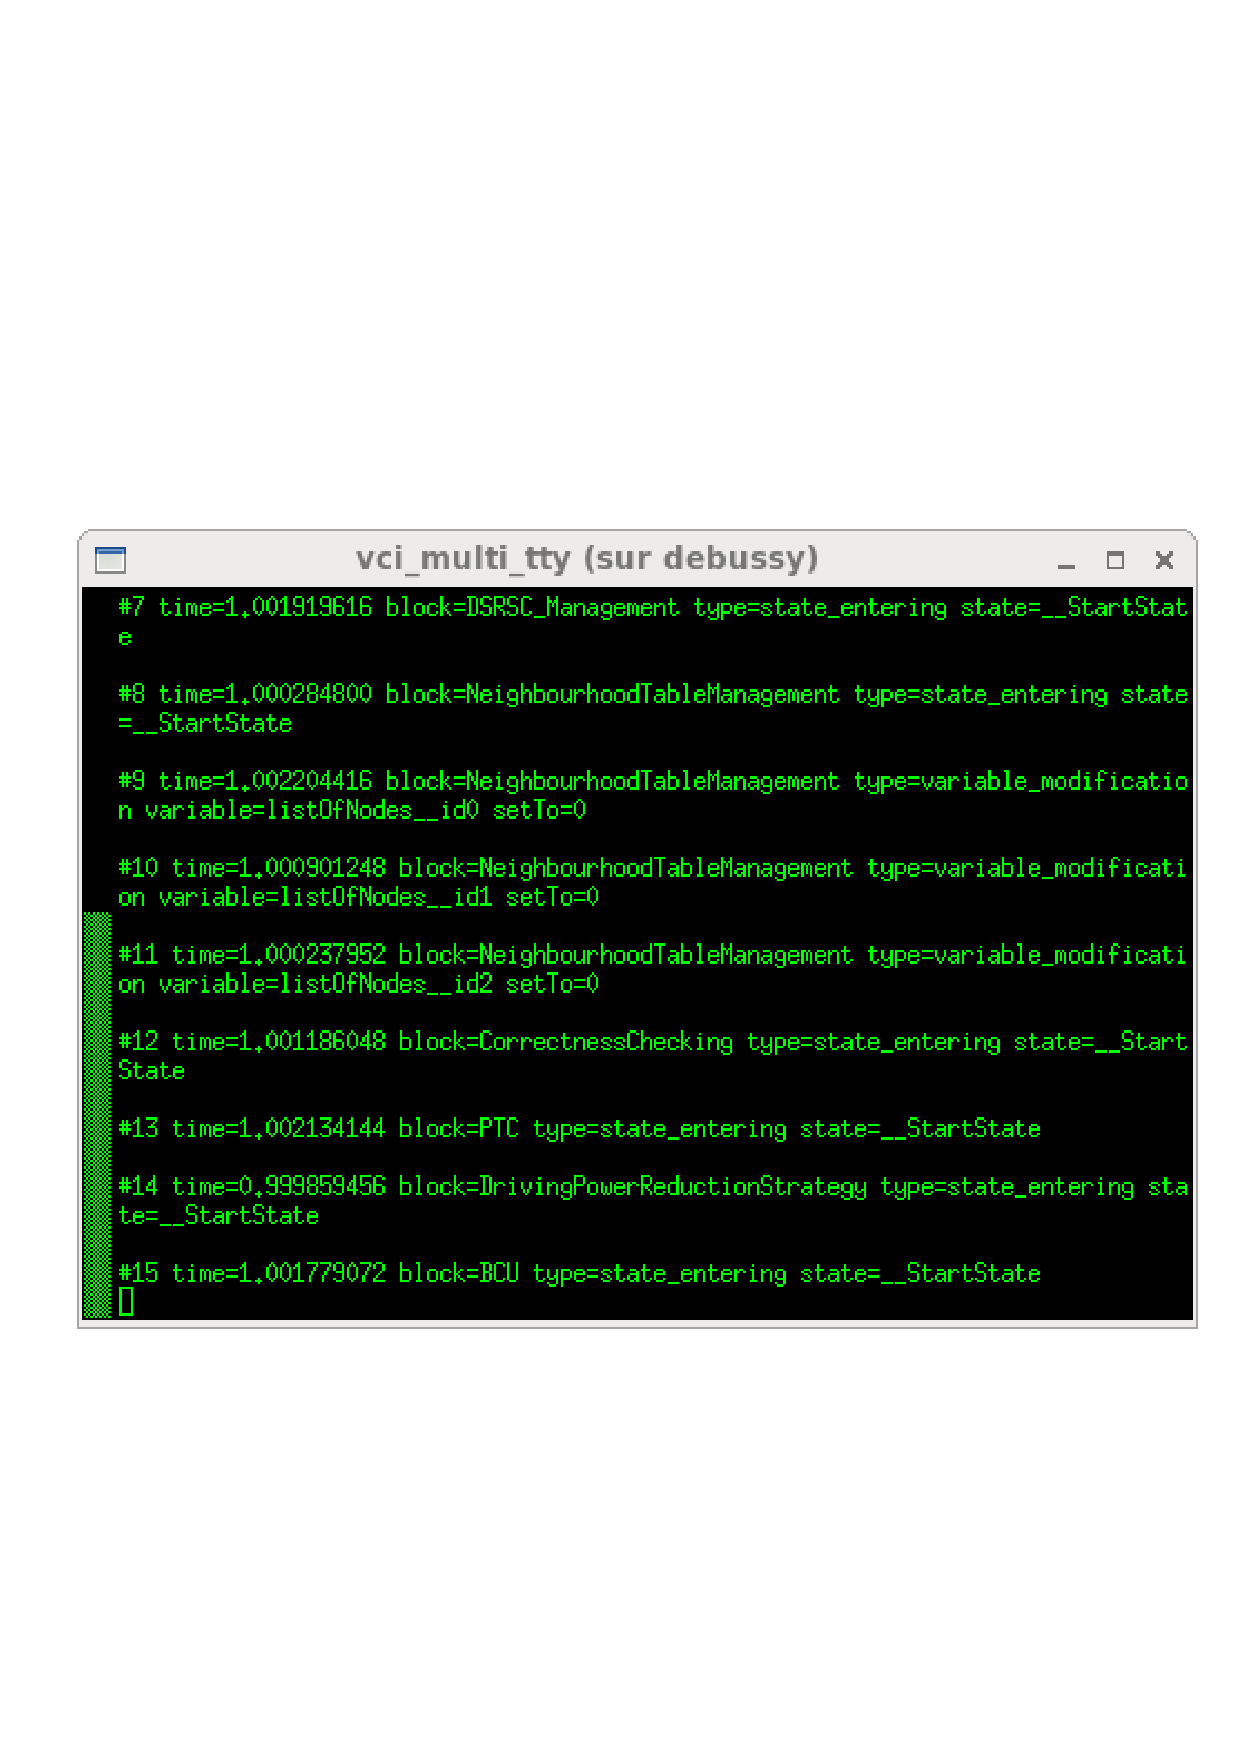
\includegraphics[width=5cm]{simu}\\
SoCLib simulation window
\end{center}
\column{7cm}
\begin{center}
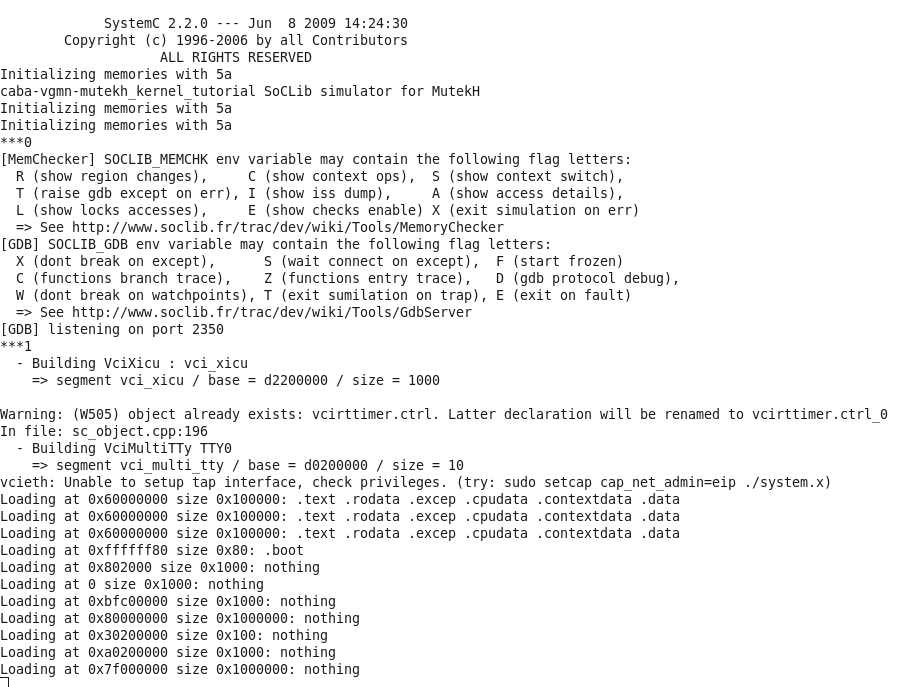
\includegraphics[width=6cm]{soclib_simu}\\
Invoking SoCLib simulation
\end{center}
\end{columns}
}

\section{Upcoming Extensions}
\subsection{Upcoming Extensions}
\frame[containsverbatim]{
\MyLogo
\frametitle{Upcoming Extensions}
\begin{itemize}
\item We will shortly supply a virtual machine for Windows
\item Adaptation to SysML-Sec \\
\texttt{http://sysml-sec.telecom-paristech.fr/}
\item Debug mode: very similar to POSIX version
\item Trace mode: cycle accurate traces of CABA Simulation
(proposed as a M2 project see \texttt{http://www-soc.lip6.fr/offres-demplois/stages/})
\end{itemize}
}

\subsection{References}

\frame[containsverbatim]{
\MyLogo
\frametitle{Web Site and Contacts}

 \texttt{http://ttool.telecom-paristech.fr} 

or 

\texttt{https://www-soc.lip6.fr/trac/avatarsoclib}

Contact daniela.genius@lip6.fr, ludovic.apvrille@telecom-paristech.fr

}

\end{document}
